\documentclass[twocolumn,twoside]{base/ajstd}

% Article information (authors ignore)
\articleinformation{Vol xx, No x, xxxx, xx–xx} % Volume, issue, year, page range
\articleinformationtruncated{xx(x): xx–xx} % Truncated volume, issue, page range
\articledoi{10.29037/ajstd.xxx} % Article DOI
\articletype{ARTICLE TYPE} % Article type
\submitted{1 Month 2000} \revised{1 Month 2000} \accepted{1 Month 2000} % Article genesis

% Article title
\title{ASEAN Journal on Science \& Technology for Development \LaTeX \,template}

% Author(s)
\author[1,\mbox{*}]{First Author}
\author[2]{Second Author}
\author[2]{Third Author}

\authorheader{Author et al.} % Author name(s) as they should appear in the header

% Author(s) affiliations
\affil[1]{First author's affiliation. Provide the full postal address, including street name and number, city, ZIP code, and country}
\affil[2]{Second and third authors' affiliation. Provide the full postal address, including street name and number, city, ZIP code, and country}
% Corresponding author
\affil[$\mbox{*}$]{Corresponding author: \href{mailto:email@address.com}{email@address.com}}

% Abstract
\abstract{The abstract should consist of a single paragraph of no more than 200 words. Provide the background and objective of the paper, the methods used, the principal results, and conclusions. Avoid using abbreviations and citations.}

% Keywords
\keywords{Alphabetical order \\ 
Maximum five keywords \\
Avoid terms already in \\
\hphantom{} the title}

% PDF metadata (authors ignore)
\makeatletter
	\hypersetup{%
		pdftitle={\@title},%
		pdfauthor={\authorheader},%
    	pdfkeywords={\keywords},%
    	pdfsubject={\abstract}%
    }
\makeatother

\makeatletter
\def\MT@warn@unknown{}
\makeatother

\begin{document}

\setcounter{page}{1}

\maketitle
\thispagestyle{firststyle}
\linenumbers % Add line numbers

\section{INTRODUCTION}

This section should briefly explain the background of the study, provide a short review of the pertinent literature, state the originality or novelty of the research, and state the research objectives.

\section{MATERIALS AND METHODS}

In research articles, the materials and methods used in the study should be described together—first the materials, and then the methods. Enough information should be provided to enable repetition of the research. For commercial sources of the materials, the name of the company, and the town and country in which they are headquartered should be indicated. To avoid an excessively long methods section, methods that have already been published should be indicated with a reference, with only the relevant modifications described.

\section{RESULTS}

Only the results of the research should be described here. Present all data as concisely as possible, in the form of tables or figures (if appropriate). 

\subsection{Tables}

Size a table to fit in a single column (Table \ref{tab:1}) or across two columns (Table \ref{tab:2}). Avoid large tables (i.e. those that fit more than a single page), unless absolutely necessary.

Every table and figure should be cited in the text in numerical order (i.e. Table 2 cannot be cited before Table 1). Place table footnotes below the table, indicating them with superscripted lowercase letters or asterisks (for significance values and other statistical data).

\subsubsection{Table captions}

Every table should have a caption that is concise but clear enough to explain its main components independently from the text. If the table contains previously published material, cite the original source at the end of the caption. If the results are expressed as a percentage, state the absolute value(s) that correspond to 100\%.

\begin{table}[b]
  	\centering\footnotesize\sffamily
  	\caption{Example single-column table.}
  	\begin{tableminipage}{\linewidth}
    	\begin{tabularx} {\linewidth}{XXX}
			\toprule
            Column 1\textsuperscript{a} & Column 2 & Column 3  \\            
	    	\midrule
            Row 1 & Row 1 & Row 1 \\
            Row 2 & Row 2 & Row 2 \\
            Row 3 & Row 3 & Row 3 \\
            Row 4 & Row 4 & Row 4 \\
            Row 5 & Row 5 & Row 5 \\
            \bottomrule
    	\end{tabularx}
        \label{tab:1}
        \vskip0pt
        \textsuperscript{a}Example footnote.
  	\end{tableminipage}
\end{table}

\begin{table*}[t]
  	\centering\footnotesize\sffamily
  	\caption{Example double-column table.}
  	\begin{tableminipage}{\linewidth}
    	\begin{tabularx} {\linewidth}{XXXXXX}
			\toprule
            Column 1 & Column 2 & Column 3 & Column 4 & Column 5 & Column 6 \\            
	    	\midrule
            Row 1 & Row 1 & Row 1 & Row 1 & Row 1 & Row 1 \\
            Row 2 & Row 2 & Row 2 & Row 2 & Row 2 & Row 2 \\
            Row 3 & Row 3 & Row 3 & Row 3 & Row 3 & Row 3 \\
            Row 4 & Row 4 & Row 4 & Row 4 & Row 4 & Row 4 \\
            Row 5 & Row 5 & Row 5 & Row 5 & Row 5 & Row 5 \\
            \bottomrule
    	\end{tabularx}
        \label{tab:2}
  	\end{tableminipage}
\end{table*}

\subsection{Figures}

Ensure that the figure will fit into either one column (Figure \ref{fig:1}) or two columns (Figure \ref{fig:2}). Images should be of sufficiently high resolution to be easily viewable when printed or on high resolution screens (minimum of 300 dpi).

Every figure should be cited in the text in numerical order (i.e. Figure 2 cannot be cited before Figure 1). Figures should be referred to as "Figure" not "Fig." Denote figure parts with lowercase letters (e.g. Figure 1a, Figure 1b).

\subsubsection{Figure formatting}

Photographs must have internal scale markers and symbols, and arrows or letters should contrast greatly with the background. Fira Sans is the recommended typeface for text within figures (if you don’t have it installed on your computer, you can download it from Google Fonts). Otherwise, a sans-serif such as Open Sans or Helvetica may be used. Where photographs of gel, autoradiograms, and so on have been processed to enhance their quality, this should be stated.

\subsubsection{Figure captions}

Every figure should have a caption that is concise but clear enough to explain its main components independently from the text. If the figure contains previously published material, cite the original source at the end of the caption.

\begin{figure}[!b]
	\centering
	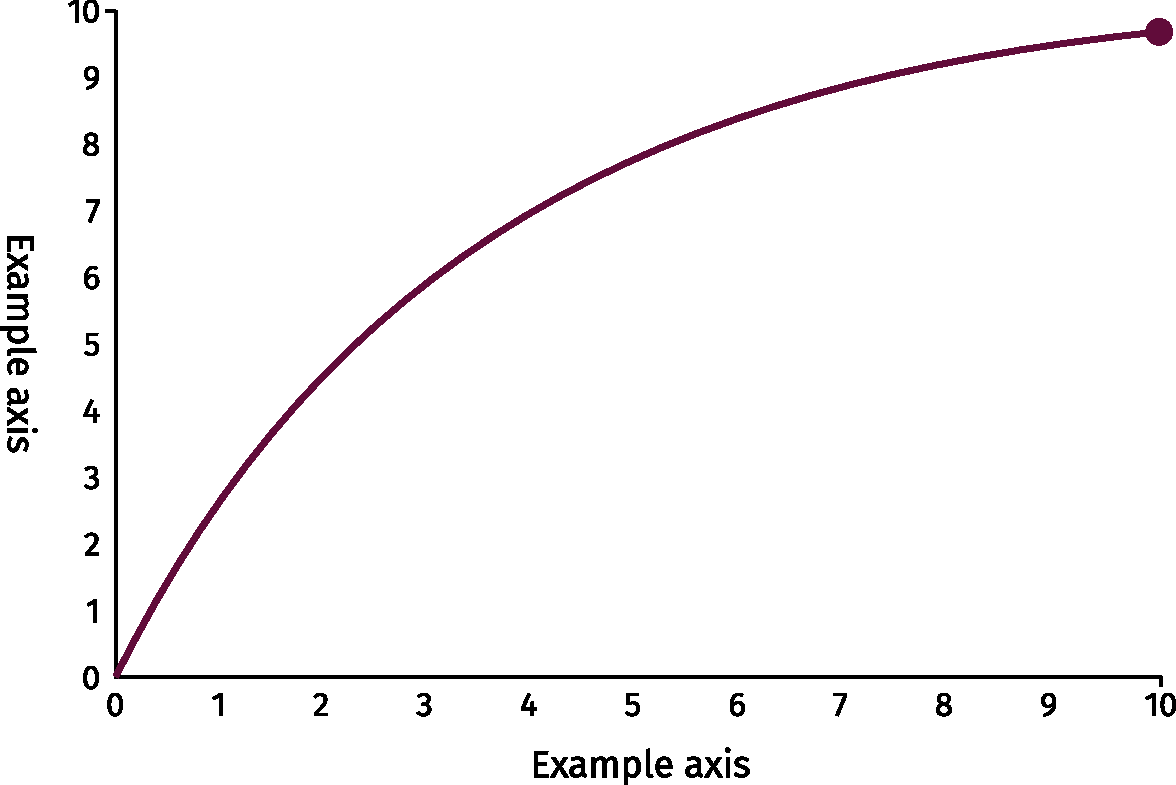
\includegraphics[width=\linewidth]{figures/Figure1.pdf}
	\caption{Example figure caption for a single-column image.}
	\label{fig:1}
\end{figure}

\begin{figure*}[!b]
	\centering
	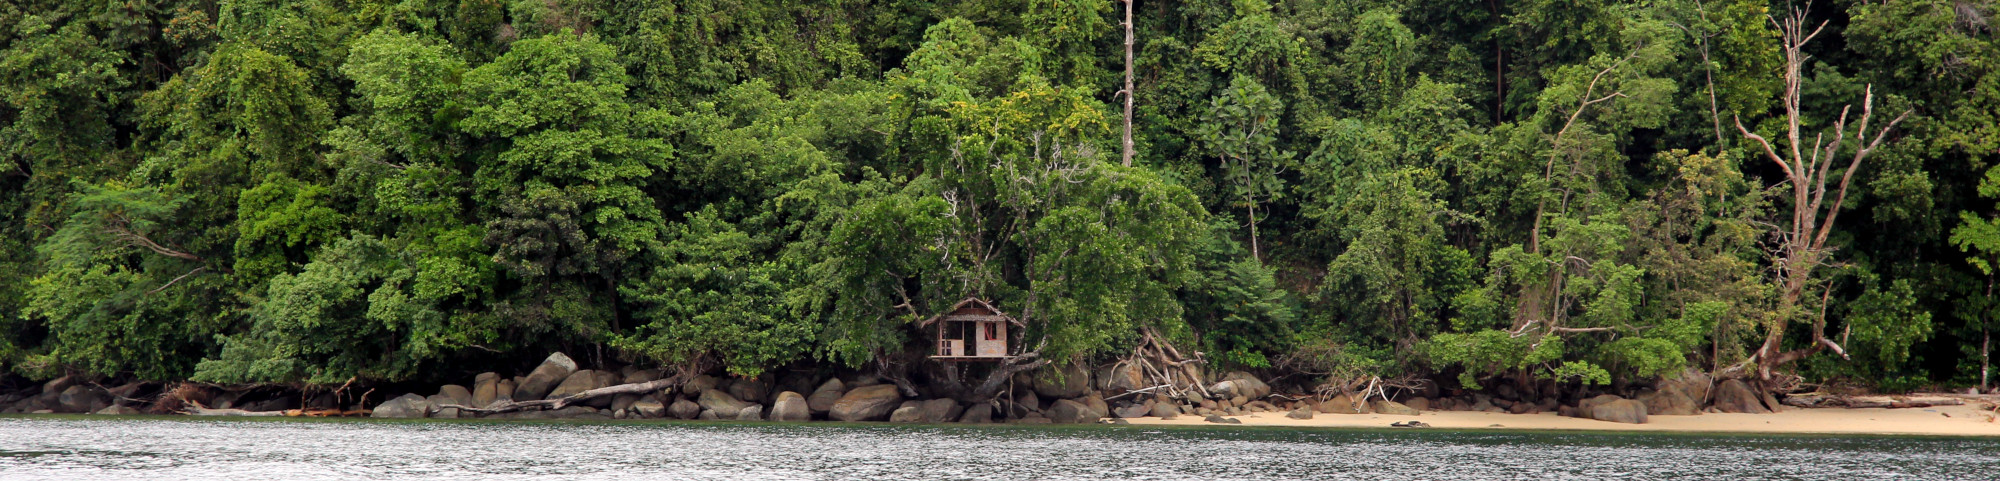
\includegraphics[width=\linewidth]{figures/Figure2.jpg}
	\caption{Example figure caption for a double-column image. Images that are wider than they are tall might be more readable as double-column figures, whereas tall images will likely take up too much page space. (Photo by Joaquim Baeta.)}
	\label{fig:2}
\end{figure*}

\section{DISCUSSION}

If necessary, it is permissible to combine this section with Results to form a Results and discussion section. Regardless, an interpretation of the results of the work in the context of previous research should be provided. Avoid simply repeating the results (that’s what the Results section is for). Also avoid excessive citations; the works being referenced must be relevant to the results being discussed.

\section{CONCLUSIONS}

Present the main conclusions of the study, along with their implications for future research or science and technology policy in the ASEAN region.

\section*{ACKNOWLEDGMENTS}

Acknowledge anyone who contributed to the research or the writing of the manuscript, as well as any funding or grants received in support of it. The names of funding organizations should be written in full, along with the grant numbers, if available. Examples of individuals you should acknowledge include people who provided assistance with study design or analysis, or guidance through a study area, or who provided advice on the language, edited, or proofread the article.

\section*{AUTHORS’ CONTRIBUTIONS}

Each author’s contribution to the research and manuscript should be noted, using only their initials to indicate their names. For example, “MP, FW designed the study. MP, LS carried out the laboratory work. MP, FW, LS, DN analyzed the data. MP, FW, DN wrote the manuscript. All authors read and approved the final version of the manuscript.”

\section*{COMPETING INTERESTS}

All competing interests—be they financial, professional, or personal relationships that are relevant to the submitted work—must be declared. If a funding source contributed to the design, data collection, analysis, or writing of the manuscript, or the decision to submit it to AJSTD, this should be clearly stated. If one or more authors have any form of—past or present—relationship with AJSTD, the extent of this relationship must be described. If one or more authors work or have worked for an organization that may benefit from the publication of the article, this must also be clearly stated. Please read AJSTD’s Publication Ethics statement to understand why it is important to acknowledge any and all competing interests.

\section*{REFERENCES AND CITATIONS}

For the purposes of efficiency and conciseness, aim for 10--25 references.

Use a reference manager such as Zotero or Mendeley to build your reference list, save the file as "references.bib", and then upload it to the \verb|references| folder. Alternatively, copy and paste the file contents into the \verb|references.bib| file. All references should be formatted in a manner compatible with BibTeX. 

A reference must be cited for it to appear in the reference list. For most cases, you only need to cite a reference in one of two ways: \\

\noindent \verb|\citet{Smith2000}| if it appears in the beginning or middle of a sentence; e.g. "\citet{Smith2000} observed that precision is important in science." \\

\noindent \verb|\citep{Smith2000}| if it appears at the end of a sentence; e.g. "In science, precision is important \citep{Smith2000}."

If you have cited and formatting your reference correctly, it will automatically appear in the reference list, as shown below.

\bibliography{references/references}

\atColsEnd{\vfill}

\end{document}